\documentclass[tikz,border=10pt]{standalone}
\usetikzlibrary{arrows.meta, positioning, shapes.geometric, shapes.misc, fit, backgrounds, calc, matrix}

\tikzset{
    >=Latex,
    font=\sffamily\large,
    node distance=1.5cm and 3cm,
    dag_result/.style={
        rectangle, 
        draw=green!70!black, 
        fill=green!15, 
        very thick, 
        minimum width=4.5cm, 
        minimum height=1.5cm, 
        text width=5cm,
        align=center
    },
    dag_lemma/.style={
        rounded rectangle, 
        draw=orange!80!black, 
        fill=yellow!20, 
        very thick, 
        minimum width=4.5cm, 
        minimum height=1.5cm, 
        text width=5cm,
        align=center
    },
    dag_model/.style={
        ellipse, 
        draw=blue!70!black, 
        fill=blue!12, 
        very thick, 
        minimum width=4.5cm, 
        minimum height=1.5cm, 
        text width=4.5cm,
        align=center
    },
    dag_unformalized/.style={
        rectangle, 
        draw=gray!60!black, 
        fill=gray!10, 
        very thick, 
        dashed, 
        minimum width=4.5cm, 
        minimum height=1.5cm, 
        text width=5cm,
        align=center
    },
    dag_conditional/.style={
        rectangle, 
        rounded corners,
        draw=orange!80!black, 
        fill=orange!10, 
        very thick, 
        minimum width=4.5cm, 
        minimum height=1.5cm, 
        text width=5cm,
        align=center
    },
    dag_partial/.style={
        rectangle,
        rounded corners,
        draw=yellow!55!black,
        fill=yellow!10,
        very thick,
        dashed,
        minimum width=4.5cm,
        minimum height=1.5cm,
        text width=5cm,
        align=center
    },
    dag_scaffold/.style={
        rectangle,
        draw=gray!55!black,
        fill=white,
        very thick,
        dotted,
        minimum width=4.5cm,
        minimum height=1.5cm,
        text width=5cm,
        align=center
    },
    dag_caveat/.style={
        diamond, 
        draw=red!70!black, 
        fill=red!10, 
        minimum width=4cm, 
        align=center, 
        inner sep=0pt, 
        font=\sffamily\small
    },
    dag_arrow/.style={
        -{Stealth[scale=1.2]}, 
        very thick,
        shorten >=1.5pt,
        shorten <=1.5pt
    },
    dag_dashed_arrow/.style={
        -{Stealth[scale=1.2]}, 
        very thick, 
        dashed,
        shorten >=1.5pt,
        shorten <=1.5pt
    },
    dag_template_legend/.style={
        minimum width=2.6cm,
        minimum height=0.8cm,
        text width=2.45cm,
        inner sep=3pt,
        font=\sffamily\small,
        align=center
    },
    dag_template_note/.style={
        rectangle,
        draw=gray!50,
        fill=gray!5,
        rounded corners,
        text width=13cm,
        align=left,
        font=\sffamily\small,
        inner sep=6pt
    }
}

% Legend Helper
\newcommand{\daglegend}[2]{
    \node[draw, rounded corners, very thick, fit=#1, inner sep=12pt, label=above:\textbf{\Large Legend}] (#2) {};
}


\begin{document}
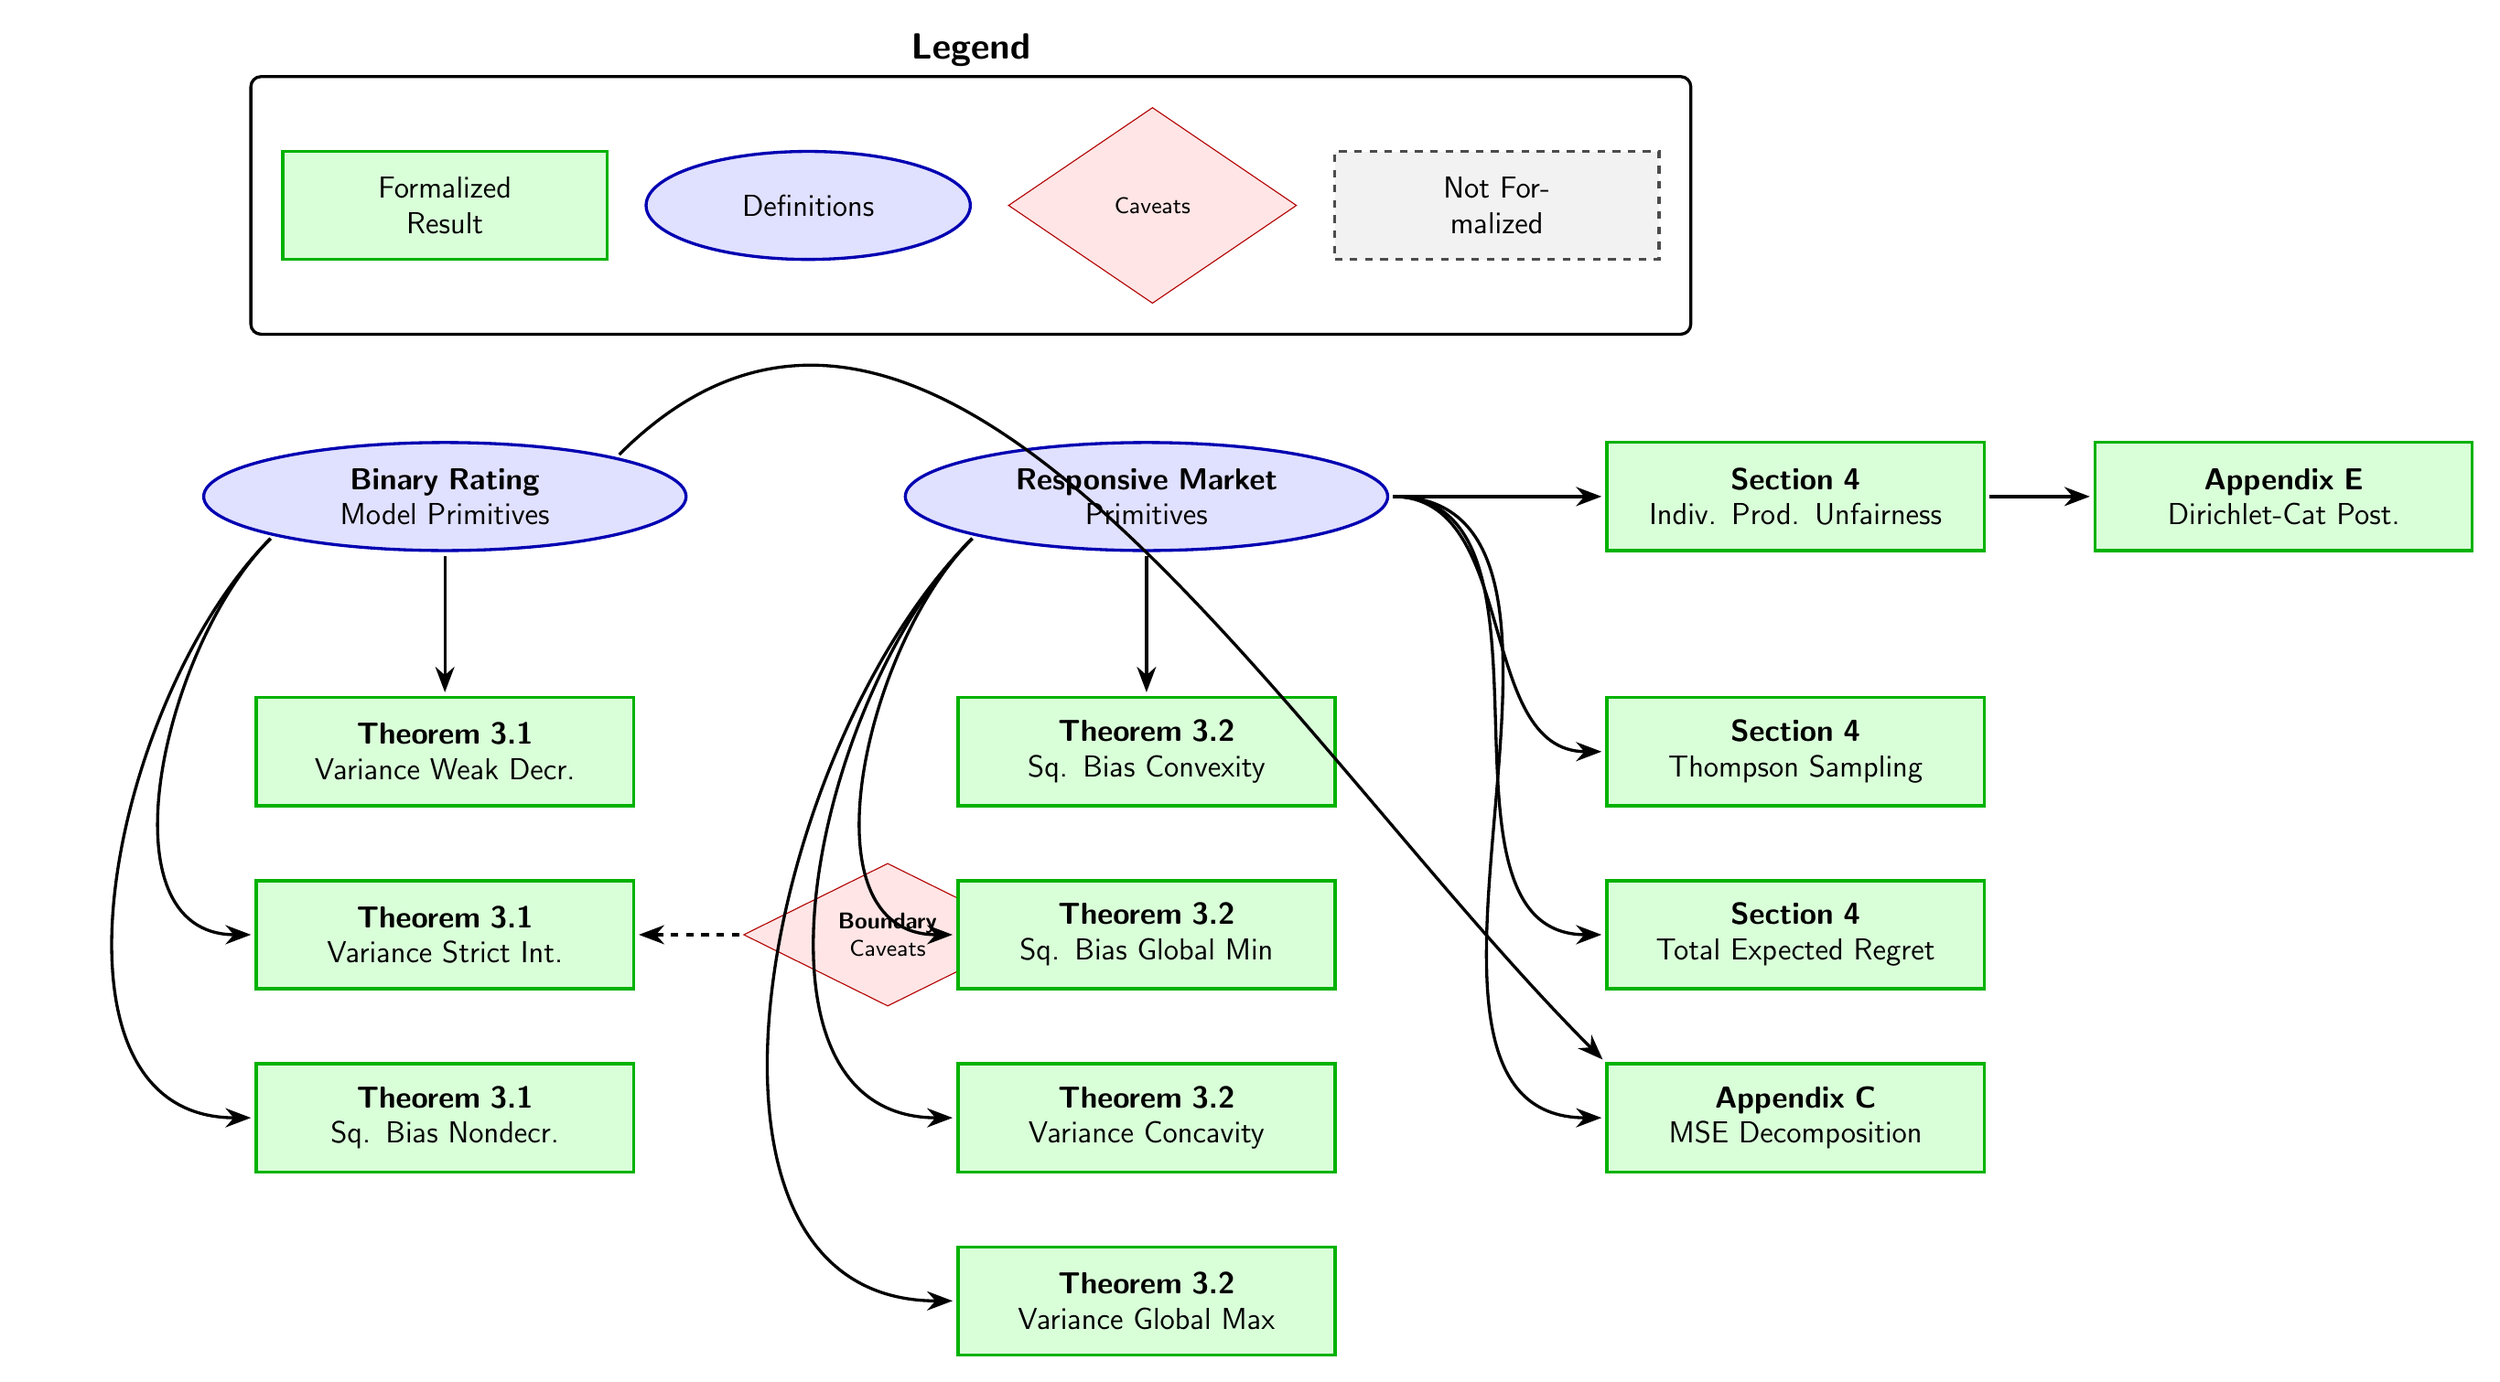
\begin{tikzpicture}

% --- Legend ---
\node[dag_result, text width=2.5cm] (legRes) {Formalized Result};
\node[dag_model, right=0.5cm of legRes, text width=2.5cm] (legDef) {Definitions};
\node[dag_caveat, right=0.5cm of legDef, text width=2.5cm] (legCav) {Caveats};
\node[dag_unformalized, right=0.5cm of legCav, text width=2.5cm] (legNot) {Not Formalized};
\daglegend{(legRes)(legDef)(legCav)(legNot)}{Legend}

% --- Column 1 (Fixed Model) ---
\node[dag_model, below=2.5cm of legRes] (ModelDefs) {\textbf{Binary Rating} \\ Model Primitives};
\node[dag_result, below=2cm of ModelDefs] (Thm3_1_Var_Weak) {\textbf{Theorem 3.1} \\ Variance Weak Decr.};
\node[dag_result, below=1cm of Thm3_1_Var_Weak] (Thm3_1_Var_Strict) {\textbf{Theorem 3.1} \\ Variance Strict Int.};
\node[dag_result, below=1cm of Thm3_1_Var_Strict] (Thm3_1_Bias) {\textbf{Theorem 3.1} \\ Sq. Bias Nondecr.};
\node[dag_caveat, right=1.5cm of Thm3_1_Var_Strict] (Boundary_Caveats) {\textbf{Boundary} \\ Caveats};

% --- Column 2 (Responsive Market) ---
\node[dag_model, right=of ModelDefs] (DynamicDefs) {\textbf{Responsive Market} \\ Primitives};
\node[dag_result, below=2cm of DynamicDefs] (Thm3_2_Bias_Convex) {\textbf{Theorem 3.2} \\ Sq. Bias Convexity};
\node[dag_result, below=1cm of Thm3_2_Bias_Convex] (Thm3_2_Bias_Min) {\textbf{Theorem 3.2} \\ Sq. Bias Global Min};
\node[dag_result, below=1cm of Thm3_2_Bias_Min] (Thm3_2_Var_Concave) {\textbf{Theorem 3.2} \\ Variance Concavity};
\node[dag_result, below=1cm of Thm3_2_Var_Concave] (Thm3_2_Var_Max) {\textbf{Theorem 3.2} \\ Variance Global Max};

% --- Column 3 (Individual Producer & Appendix) ---
\node[dag_result, right=of DynamicDefs] (Unfairness) {\textbf{Section 4} \\ Indiv. Prod. Unfairness};
\node[dag_result, below=2cm of Unfairness] (Thompson) {\textbf{Section 4} \\ Thompson Sampling};
\node[dag_result, below=1cm of Thompson] (Regret) {\textbf{Section 4} \\ Total Expected Regret};
\node[dag_result, below=1cm of Regret] (MSE_Decomp) {\textbf{Appendix C} \\ MSE Decomposition};
\node[dag_result, right=1.5cm of Unfairness] (Dirichlet) {\textbf{Appendix E} \\ Dirichlet-Cat Post.};

% --- Edges ---
\draw[dag_arrow] (ModelDefs) -- (Thm3_1_Var_Weak);
\draw[dag_arrow] (ModelDefs.south west) to[out=225, in=180] (Thm3_1_Var_Strict.west);
\draw[dag_arrow] (ModelDefs.south west) to[out=225, in=180] (Thm3_1_Bias.west);
\draw[dag_dashed_arrow] (Boundary_Caveats) -- (Thm3_1_Var_Strict);

\draw[dag_arrow] (DynamicDefs) -- (Thm3_2_Bias_Convex);
\draw[dag_arrow] (DynamicDefs.south west) to[out=225, in=180] (Thm3_2_Bias_Min.west);
\draw[dag_arrow] (DynamicDefs.south west) to[out=225, in=180] (Thm3_2_Var_Concave.west);
\draw[dag_arrow] (DynamicDefs.south west) to[out=225, in=180] (Thm3_2_Var_Max.west);

\draw[dag_arrow] (DynamicDefs) -- (Unfairness);
\draw[dag_arrow] (DynamicDefs.east) to[out=0, in=180] (Thompson.west);
\draw[dag_arrow] (DynamicDefs.east) to[out=0, in=180] (Regret.west);
\draw[dag_arrow] (DynamicDefs.east) to[out=0, in=180] (MSE_Decomp.west);
\draw[dag_arrow] (Unfairness) -- (Dirichlet);
\draw[dag_arrow] (ModelDefs.north east) to[out=45, in=135] (MSE_Decomp.north west);

\end{tikzpicture}
\end{document}
